\documentclass[11pt,a4paper]{article}
%--------------------------------------------------
%Packages bases
\usepackage{lmodern}
\usepackage[spanish]{babel}
\usepackage[utf8]{inputenc}
\usepackage{array}
\usepackage{ifthen}
\usepackage{transparent}
\usepackage{eso-pic}
\usepackage{multirow}
\usepackage{afterpage}
\usepackage{amsfonts}
\usepackage{amssymb}
\usepackage{amsthm}
\usepackage{float}
\usepackage{ifthen}
\usepackage{framed}
\usepackage{xspace}
\usepackage{multicol}
\usepackage{enumitem}
\usepackage{color}
\usepackage{titlesec}
\usepackage{ifthen}


%----------------------------------------
%design
\usepackage{amsmath,tikz}
\usepackage{verbatim}
\usetikzlibrary{shapes.geometric}
\usetikzlibrary{arrows}

%----------------------------------------
%color
\usepackage{transparent}
\usepackage{colortbl}
\definecolor{darkred}{rgb}{.7,0.03,0.22}
\definecolor{red_tab}{rgb}{0.96,0.88,0.86}
\definecolor{darkblue}{HTML}{0000CC}
\definecolor{vdarkblue}{HTML}{000066}
\definecolor{texte}{HTML}{660099}
\definecolor{comt}{HTML}{009933}
%-----------------------------------------


%------------------------------------------
%counters
\newcounter{step}
\newcounter{substep}
\setcounter{step}{0}
\setcounter{substep}{0}
%------------------------------------------

\usepackage{tabularx}
\usepackage{makecell}


\newcolumntype{R}[1]{>{\raggedleft\arraybackslash }p{#1}}
\newcolumntype{L}[1]{>{\raggedright\arraybackslash }p{#1}}
\newcolumntype{C}[1]{>{\centering\arraybackslash }p{#1}}

\usepackage{wasysym}


\usepackage{ifluatex}
\ifluatex
\usepackage{fontspec}
\usepackage{polyglossia}
\setdefaultlanguage{french}
\else
\usepackage[utf8]{inputenc}
\usepackage[T1]{fontenc}
\usepackage{babel}


%-----------------------------------------
%format page
\usepackage[a4paper,left=2cm,right=1cm,top=0.5cm,bottom=1cm,headheight=0cm, headsep=0cm, footskip=0cm,includefoot,includehead]{geometry}

%----------------------------------------
%footnote and header number
\usepackage{fancyhdr}
\usepackage[pages=all]{background}
\pagestyle{fancy}
\renewcommand{\headrulewidth}{0pt}
\fancyhf {} % clear all headers and footers

% Header is used to include the page background
\backgroundsetup{
scale=1,
color=black,
opacity=1,
angle=0,
contents={%
  
\includegraphics[width=\paperwidth,height=\paperheight]{images/paper.jpg}
  }%
}

%-----------------------------------------
%Hyperlink
\usepackage[colorlinks, bookmarks, linkcolor=black, citecolor=black, urlcolor=blue]{hyperref}

%-----------------------------------------
%Set Monospace font
% \usepackage{everysel}
%     \renewcommand*\familydefault{\ttdefault}
%     \EverySelectfont{%
%     \fontdimen2\font=0.4em  % interword space
%     \fontdimen3\font=0.2em  % interword stretch
%     \fontdimen4\font=0.1em  % interword shrink
%     \fontdimen7\font=0.1em  % extra space
%     \hyphenchar\font=`\-    % to allow hyphenation
% }
%-----------------------------------------
%Configurations
\newcommand{\Style}[1]{
\ifthenelse{#1=1}{\makeatletter
\newcommand{\PrepTime}[1]{\def\@PrepTime{#1\xspace}
\def\PrepTimeb{#1}}
\newcommand{\CookingTime}[1]{\def\@CookingTime{#1\xspace}}
\newcommand{\background}[1]{%
\AddToShipoutPictureBG{\AtPageLowerLeft{\transparent{0.1}\includegraphics[width=\paperwidth,height=\paperheight]{#1}}}
}
\newcommand{\CookingTempe}[1]{%
\ifnum0=#1\relax
   \def\@CookingTempe{} 
\else
  \def\@CookingTempe{-- #1$^{\circ}$} 
\fi
}

\newcommand{\TypeCooking}[1]{\def\@TypeCooking{#1}}
\newcommand{\NPerson}[1]{\def\@NbPerson{#1\xspace}}
\newcommand{\Image}[2]{\def\@ImageDim{#1} \def\@ImagePath{#2}}
\def\maketitle{%

\vspace*{0.05cm}
\begin{center}
{\Huge \@title}
\end{center}
}

\newenvironment{ingredient}
  {\noindent\begingroup\edef\x{\endgroup\noexpand}\x
  \maketitle
  
  \begin{footnotesize}\noindent\setlength\arrayrulewidth{2pt}\begin{tabular}{|L{0.62\linewidth}|L{0.33\linewidth}|}\hline\vspace{-0.21cm}\underline{\textbf{{\normalsize Ingredients (\@NbPerson persons):}}} &\\
  \begin{minipage}{\linewidth}
  \vspace{0.2cm}
  }
  {\vspace{-0.2cm}
  \end{minipage}& \vspace{-1.8cm}Preparation time: \begin{tikzpicture}
  \pgfmathsetmacro{\timeor}{\PrepTimeb}
  \ifthenelse{\timeor>60}{
  \pgfmathsetmacro{\timeorb}{90-(\PrepTimeb-60)/60*360}
  \fill[orange] (0,0.55) arc(90:-270:0.55)      -- ++(-270:-0.55)
  arc(-270:0:0)    -- cycle;
  \fill[red] (0,0.55) arc(90:\timeorb:0.55)      -- ++(\timeorb:-0.55)
  arc(\timeorb:0:0)    -- cycle;
  }{
  \pgfmathsetmacro{\timeorb}{90-(\PrepTimeb)/60*360}
  \fill[green] (0,0.55) arc(90:\timeorb:0.55)      -- ++(\timeorb:-0.55)
  arc(\timeorb:0:0)    -- cycle;
  }
  \node[fill=white,inner sep=0pt] at (0,0) {{\tiny \PrepTimeb~min}};
  \fill[black!50,even odd rule] (0,0) circle(0.65) circle(0.6);
  \fill[black!50,even odd rule] (0,0.5) circle(0.05);
  \fill[black!50,even odd rule] (0.5,0) circle(0.05);
  \fill[black!50,even odd rule] (0,-0.5) circle(0.05);
  \fill[black!50,even odd rule] (-0.5,0) circle(0.05);
  \end{tikzpicture} \par
  \vspace{0.2cm} Cooking: \@CookingTime min \@CookingTempe

  
   \par \vspace{0.2cm} Cooking Type: \@TypeCooking \\\hline\end{tabular}\vspace{0.5cm} \end{footnotesize}}


\newenvironment{main}
  {\begin{multicols}{2}
  \begin{itemize}[label=$$]
  }
  {\end{itemize}\end{multicols}}
  
\newenvironment{subingredient}[1]
{\vspace{-0.3cm}\hspace{0.5cm}\underline{#1:}
\vspace{-0.3cm}\begin{multicols}{2}
\begin{itemize}[label=$$]
}
{\end{itemize}\end{multicols}}


\newenvironment{recipe}
{
}
{}
\makeatother

%-----------------------------------------
%New environments

\newenvironment{notes}
{\vfill\def\FrameCommand{\fboxsep=\FrameSep\fbox}%
\MakeFramed {\advance\hsize-\width \FrameRestore}
\noindent\underline{\textbf{Notes and tips:}}%

\vspace{0.25cm}
\noindent\hspace{-0.15cm}}
{\vspace{2.5cm}\endMakeFramed}
  
  
\newcommand{\step}[1]{\ifthenelse{\value{step}=0}{\noindent{\large \underline{\textbf{Preparation:}}}\vspace{0.3cm}

}{}
\noindent\stepcounter{step}\setcounter{substep}{0}\the\value{step}. #1\vspace{0.3cm}

} 

\newcommand{\substep}[2][1]{\ifthenelse{\value{substep}=0}{\noindent\stepcounter{step}\the\value{step}. \underline{\textbf{#1:}}\vspace{0.3cm}

}{}
\hspace{0.3cm}\begin{minipage}{0.948\textwidth}
\noindent\stepcounter{substep}\roman{substep}. #2\vspace{0.5cm}
\end{minipage}

}   }{}
\ifthenelse{#1=2}{\makeatletter
\newcommand{\PrepTime}[1]{\def\@PrepTime{#1\xspace}
\def\PrepTimeb{#1}}
\newcommand{\CookingTime}[1]{\def\@CookingTime{#1\xspace}}
\newcommand{\background}[1]{%
\AddToShipoutPictureBG{\AtPageLowerLeft{\transparent{0.1}\includegraphics[width=\paperwidth,height=\paperheight]{#1}}}
}
\newcommand{\CookingTempe}[1]{%
\ifnum0=#1\relax
   \def\@CookingTempe{} 
\else
  \def\@CookingTempe{-- #1$^{\circ}$} 
\fi
}

\newcommand{\TypeCooking}[1]{\def\@TypeCooking{#1}}
\newcommand{\NPerson}[1]{\def\@NbPerson{#1\xspace}}
\newcommand{\Image}[2]{\def\@ImageDim{#1} \def\@ImagePath{#2}}
\def\maketitle{%

\vspace*{0.05cm}
\begin{center}
{\Huge \@title}
\end{center}
}

\newenvironment{ingredient}
  {\noindent\begingroup\edef\x{\endgroup\noexpand}\x
  \maketitle
  
  \begin{footnotesize}\noindent\setlength\arrayrulewidth{2pt}\begin{tabular}{|L{0.62\linewidth}|L{0.33\linewidth}|}\hline\vspace{-0.21cm}\underline{\textbf{{\normalsize Ingredientes (\@NbPerson personas):}}} &\\
  \begin{minipage}{\linewidth}
  \vspace{0.2cm}
  }
  {\vspace{-0.2cm}
  \end{minipage}& \vspace{-1.8cm}Tiempo de preparación: \begin{tikzpicture}
  \pgfmathsetmacro{\timeor}{\PrepTimeb}
  \ifthenelse{\timeor>60}{
  \pgfmathsetmacro{\timeorb}{90-(\PrepTimeb-60)/60*360}
  \fill[orange] (0,0.55) arc(90:-270:0.55)      -- ++(-270:-0.55)
  arc(-270:0:0)    -- cycle;
  \fill[red] (0,0.55) arc(90:\timeorb:0.55)      -- ++(\timeorb:-0.55)
  arc(\timeorb:0:0)    -- cycle;
  }{
  \pgfmathsetmacro{\timeorb}{90-(\PrepTimeb)/60*360}
  \fill[green] (0,0.55) arc(90:\timeorb:0.55)      -- ++(\timeorb:-0.55)
  arc(\timeorb:0:0)    -- cycle;
  }
  \node[fill=white,inner sep=0pt] at (0,0) {{\tiny \PrepTimeb~min}};
  \fill[black!50,even odd rule] (0,0) circle(0.65) circle(0.6);
  \fill[black!50,even odd rule] (0,0.5) circle(0.05);
  \fill[black!50,even odd rule] (0.5,0) circle(0.05);
  \fill[black!50,even odd rule] (0,-0.5) circle(0.05);
  \fill[black!50,even odd rule] (-0.5,0) circle(0.05);
  \end{tikzpicture} \par
  \vspace{0.2cm} Cocción: \@CookingTime min \@CookingTempe

   \par \vspace{0.2cm} Tipo de cocción: \@TypeCooking \\\hline\end{tabular}\vspace{0.5cm} \end{footnotesize}}


\newenvironment{main}
  {\begin{multicols}{2}
  \begin{itemize}[label=$$]
  }
  {\end{itemize}\end{multicols}}
  
\newenvironment{subingredient}[1]
{\vspace{-0.3cm}\hspace{0.5cm}\underline{#1:}
\vspace{-0.3cm}\begin{multicols}{2}
\begin{itemize}[label=$$]
}
{\end{itemize}\end{multicols}}


\newenvironment{recipe}
{
}
{}
\makeatother

%-----------------------------------------
%New environments

\newenvironment{notes}
{\vfill\def\FrameCommand{\fboxsep=\FrameSep\fbox}%
\MakeFramed {\advance\hsize-\width \FrameRestore}
\noindent\underline{\textbf{Notas y tips:}}%

\vspace{0.25cm}
\noindent\hspace{-0.15cm}}
{\vspace{1cm}\endMakeFramed}
  
  
\newcommand{\step}[1]{\ifthenelse{\value{step}=0}{\noindent{\large \underline{\textbf{Preparación:}}}\vspace{0.3cm}

}{}
\noindent\stepcounter{step}\setcounter{substep}{0}\the\value{step}. #1\vspace{0.3cm}

} 

\newcommand{\substep}[2][1]{\ifthenelse{\value{substep}=0}{\noindent\stepcounter{step}\the\value{step}. \underline{\textbf{#1:}}\vspace{0.3cm}

}{}
\hspace{0.3cm}\begin{minipage}{0.948\textwidth}
\noindent\stepcounter{substep}\roman{substep}. #2\vspace{0.5cm}
\end{minipage}

}   }{}}



\newcommand{\asignatura}{Sistemas Electrónicos}
\newcommand{\actividad}{Tareas puntuables}
\newcommand{\titulo}{\textbf{Virtex-6} de Xilinx}
\newcommand{\subtitulo}{Tarea \# 2}
\newcommand{\foto}{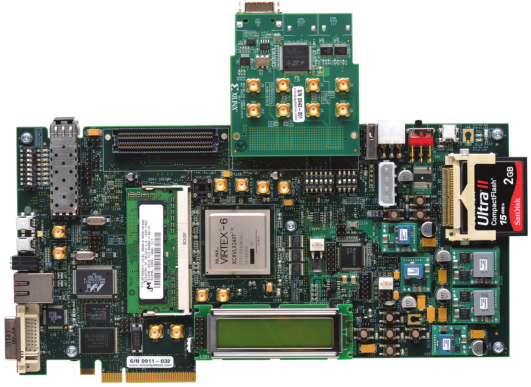
\includegraphics[scale=1.2]{images/virtex6.pdf}}
\newcommand{\descripcion}{Resumen sobre las características más destacadas de la FPGA \textbf{Virtex-6} de Xilinx.}
\newcommand{\curso}{2021-2022}
\newcommand{\autor}{Jorge Benavides Macías }
\begin{document}
%%%%%%%%%%%%%%%%%%%%%%%%%%%%%%%%%%%%%%%%%%%%%%%%%%%%%%%%%%%%%%%%%%%%%%%%
% Plantilla TFG/TFM
% Escuela Politécnica Superior de la Universidad de Alicante
% Realizado por: Jose Manuel Requena Plens
% Contacto: info@jmrplens.com / Telegram:@jmrplens
%%%%%%%%%%%%%%%%%%%%%%%%%%%%%%%%%%%%%%%%%%%%%%%%%%%%%%%%%%%%%%%%%%%%%%%%


\begin{titlepage}

% Márgenes de esta pagina modificados
\newgeometry{ignoreall,top=2cm,bottom=2cm}
\setlength{\centeroffset}{-0.5\oddsidemargin}
\addtolength{\centeroffset}{0.5\evensidemargin}
\thispagestyle{empty}

\AddToShipoutPictureBG*{%
\begin{tikzpicture}[overlay,remember picture]
\draw[line width=10pt]
    ($ (current page.north west) + (2cm,-2cm) $)
    rectangle
    ($ (current page.south east) + (-2cm,2cm) $);
\draw[line width=1.5pt]
    ($ (current page.north west) + (2.2cm,-2.2cm) $)
    rectangle
    ($ (current page.south east) + (-2.2cm,2.2cm) $);
\end{tikzpicture}
}

\FuenteTitulo
\centering
\vspace*{5em}
{\fontsize{30pt}{0pt}\selectfont \seguridadx}
\vfill
{\fontsize{25pt}{0pt}\selectfont \identificadorx}
\vfill
{\fontsize{25pt}{0pt}\selectfont \organizacionx}
\vfill
{\fontsize{25pt}{0pt}\selectfont \ul\titulox}
\vfill
% {\fontsize{20pt}{0pt}\selectfont \subtitulox}
% \vfill
{\fontsize{20pt}{0pt}\selectfont \autorx}

\vspace{1em}
{\fontsize{15pt}{0pt}\selectfont \asociacionx}
\vfill
{\fontsize{10pt}{0pt}\selectfont \fechax}
\vfill
{\fontsize{25pt}{0pt}\selectfont \tipox}
\vfill
{\fontsize{30pt}{0pt}\selectfont \seguridadx}
\vspace*{5em}
\vfill

% \def\FuenteTamano{50pt}
% % Titulo y subtitulo
% \vspace*{5em}
% \def\FuenteTamano{30pt}
% {\FuenteTitulo\fontsize{\FuenteTamano}{0pt}\selectfont\color{black} \seguridadx}
% \vfill
% \def\FuenteTamano{25pt}
% {\FuenteTitulo\fontsize{\FuenteTamano}{0pt}\selectfont\color{black} \identificadorx}
% \vfill
% {\FuentePortada \fontsize{\TamTrabajo}{35pt}\selectfont\color{black}\organizacionx}
% \vfill
% {\raggedright{\FuenteTitulo\fontsize{\FuenteTamano}{35pt}\selectfont\color{black} \titulox}}
% \vfill
% % {\raggedright{\FuenteTitulo\fontsize{\FuenteTamano}{110pt}\selectfont\color{black} \subtitulox }}
% % \vfill
% {\FuentePortada \fontsize{\TamTrabajo}{25pt}\selectfont\color{black} \autorx}
% \vfill
% {\FuentePortada \fontsize{\TamOtros}{30pt}\selectfont\color{black}\fechax}
% \vfill
% {\FuentePortada \fontsize{\TamTrabajo}{30pt}\selectfont\color{black}\tipox}
% \vfill
% \def\FuenteTamano{30pt}
% {\FuenteTitulo\fontsize{\FuenteTamano}{0pt}\selectfont\color{black} \seguridadx}
% \vspace{2cm}
% \vfill
\end{titlepage}

% A partir de aquí aplica los márgenes establecidos en configuracioninicial.tex
\restoregeometry

La \textbf{Virtex-6} es una FPGA, de la compañía Xilinx, orientada al alto rendimiento, sus 3 subfamilias de propósito general (LXT), procesamiento digital de señales (SXT) y mayor ancho de banda (HXT) son la prueba, la diferencia entre las subfamilias es la cantidad de componentes que tienen de algún dispositivo específico, por ejemplo el modelo dedicado al procesamiento de señales hará más operaciones por lo tanto necesitará más procesadores de señales (DSP48E1), el modelo HXT por su utilidad en la comunicación necesitará más \textit{SerDes} para transmitir correctamente los datos a altas velocidades y el de propósito general más Slices.

\begin{figure}[h]
    \centering
    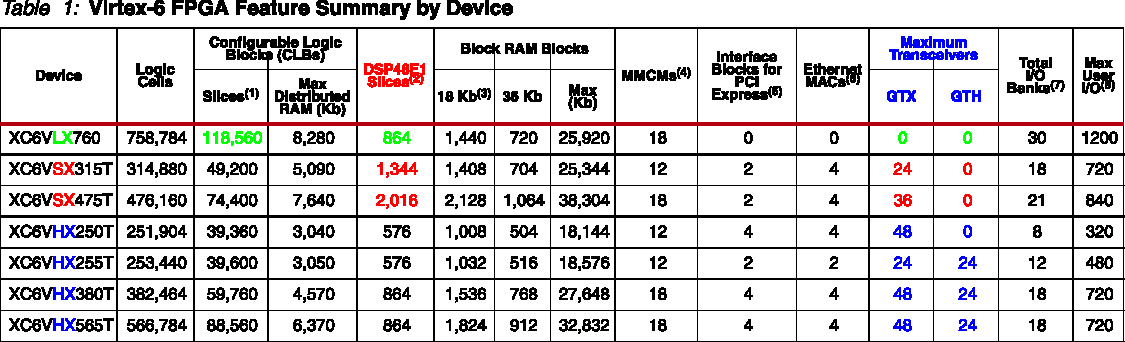
\includegraphics[scale=0.75]{images/Virtex-6 FPGA feature summary.pdf}
    \caption{Tabla con las subfamilias de la \textbf{Virtex-6} y sus diferencias}
\end{figure}

Como detalle ``curioso'' los bloques de RAM siempre son de 36Kbits pero pueden usarse como dos independientes de 18Kbits.

{\Large \textbf{CLBs, Slices y LUTs}}

Las CLBs de la \textbf{Virtex-6} son muy parecidas a las de la Spartan-6 vistas en clase ya que presenta dos slices en diagonal, como se puede observa en la figura \ref{fig:slice_scheme} la conexión entre las Slices de distintas CLBs es vertical, manteniendo fija al columna. Cada Slice contiene 4 LUTs, 8 biestables tipo D, multiplexores y lógica de acarreo. Las SlicesM tienen RAM distribuida y registros de desplazamiento.\par
\begin{wrapfigure}{r}{0.3\textwidth} 
    \centering
    \dummypic{scale = 0.45}{images/slice_scheme.pdf}{Relación entre las filas y columnas de las CLBs y Slices}{fig:slice_scheme}
\end{wrapfigure}\par
 Las LUTs tiene 6 entradas y 2 salidas, se pueden implementar funciones complejas de hasta 6 entradas por LUT e incluso \textbf{soporta dos funciones distintas de 5 entradas}, los multiplexores que contienen pueden usarse para generar funciones de 7 y 8 entradas, para funciones más grandes se combinan varias slices. \textbf{No hay conexión directa entre las slices para generar funciones de más de 8 entradas}.

En la figura \ref{fig:bioestable} se observa que vienen con 4 funciones extra, puesta a 0 o a 1 en el inicio o forzar el cambio a 0 o a 1, es un detalle importante ya que en nuestros circuitos metemos un reset para iniciar los flip-flops y que almacenen un valor, con estas funciones se pueden omitir pasos y que el circuito inicie más rápido.
\begin{wrapfigure}{l}{0.25\textwidth}
  \vspace{-0.05\textwidth}
    \dummypic{scale=1}{images/biestable_tipo_d.pdf}{Biestable tipo D}{fig:bioestable}
    \vspace*{-0.05\textwidth}
\end{wrapfigure}

 Como he comentado antes las LUTs de \textbf{las SlicesM se pueden usar para generar bloques de memoria RAM}, se caracteriza por tener una escritura síncrona, además tienen hasta 11 modos distintos de configuración caracterizado por el tipo de puerto y la cantidad de bits que puede gestionar, \textbf{la lectura es asíncrona} pero puede hacerse síncrona utilizando algún tipo de almacenamiento en el Slice.
 
El número de LUTs para realizar cualquier bloque de memoria es como máximo de 4 LUTs que comparado con el número de LUTs necesarios para realizar un multiplicador básico es insignificante, asi que puede ser una buena opción si nos falta memoria RAM.\par

Podemos implementar memoria ROM si necesitamos cargar un programa de arranque del sistema o cargar constantes para ciertas operaciones (logaritmos, senos, cosenos, etc...), se pueden usar tanto las SlicesM como las SlicesL, por cada LUT se pueden implementar 8 bytes, las configuraciones son de 1, 2 y 4 LUTs.\par
 \begin{wrapfigure}{r}{0.35\textwidth}
    \flushleft
    \vspace*{-0.05\textwidth}
    \dummypic{scale=0.55}{images/registro_32_bits.pdf}{Configuración de un registro de 32 bits}{fig:register}
\end{wrapfigure}\par
La creación de registros, disponible en la SliceM, es un poco más complicada que la memoria RAM ya que requiere compensación en retardos y latencia, producidos tanto por las LUTs como por el tipo de conexión ya que no hay una conexión directa entre los Slices.

La técnica de balanceo de caminos combinacionales usando flip-flops es lo que resuelve el problema incluso en los esquema del datasheet el flip-flop lo pone como opcional ya que queda a criterio de las necesidades del diseñador.

Los multiplexores se pueden implementar como 4:1,8:1 y 16:1 en una sola slice.
La lógica de acarreo es en cascada, se usa para la suma y la resta, lo que aumenta el rendimiento de las operaciones por estar incluida en la Slice, cuenta con 10 entradas y 8 salidas ambas independientes. Detalle importante es que la propagación del retardo de un sumador aumenta linealmente con el número de bits porque contiene más lógica de acarreo en cascada.

{\Large \textbf{Clocking Resources}}

Para el reloj, al menos en esta versión, se ha creado un concepto nuevo llamado regiones, el número de regiones depende del tamaño de la FPGA, oscila entre 6 y 18 en las más grandes, cada región está compuesta por ``40 CLBs high'' con un reloj horizontal en una fila en el centro; también diferencia entre relojes globales, de región y de entrada/salida.

Las 32 lineas globales de reloj alimentan todos los dispositivos de la placa, en la línea del reloj solo hay un buffer para activar y desactivar la línea esto es para minimizar los efectos de retraso en las líneas más largas; 12 de las 32 líneas generales son para regiones y pueden ser arbitrarias por lo que podemos seleccionar las líneas que menos retraso generen en nuestro circuito.

La \textbf{Virtex-6}, además de la estructura de árbol global que tiene, cuenta con una red de relojes regionales los cuales son distribuidos mediante buffers (BUFRs), estas redes se caracterizan por ser low-skew y de baja potencia de funcionamiento.

\begin{figure}[H]
    \centering
    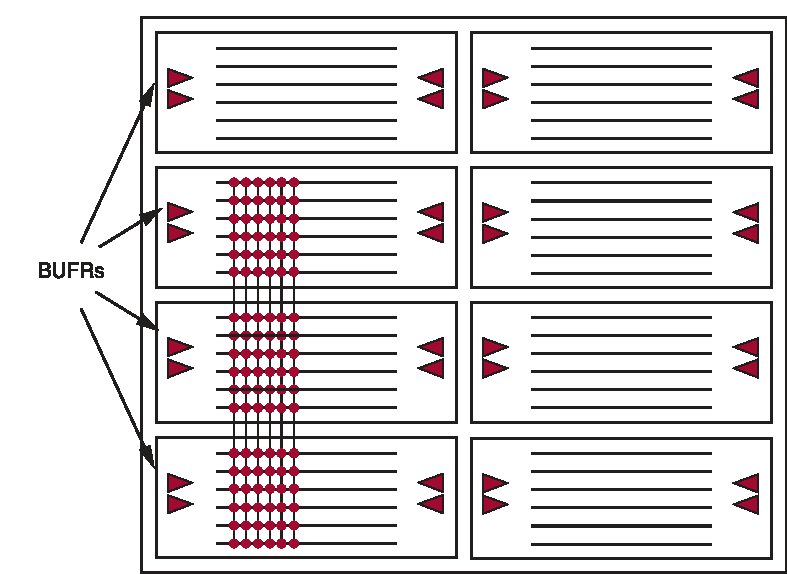
\includegraphics[scale=0.6]{images/region_net_clock.pdf}
    \caption{Buffer conduciendo el reloj a múltiples regiones}
    \label{fig:buffer}
\end{figure}

{\Large \textbf{DSP48E1 Slice}}

\begin{figure}[h]
    \centering
    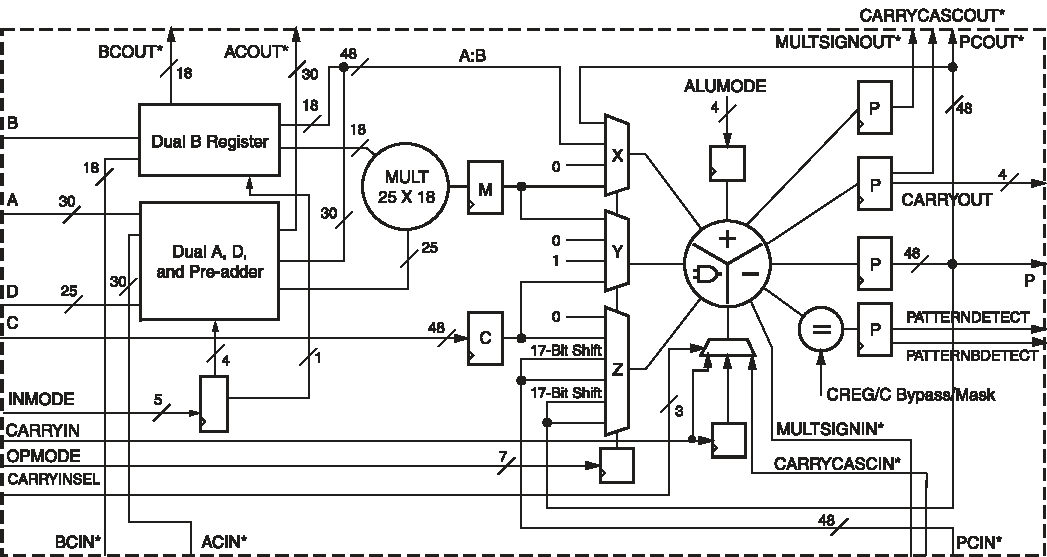
\includegraphics[scale=0.6]{images/DSP48E1.pdf}
    \caption{\textbf{Virtex-6} FPGA DSP48E1 Slice}
    \label{fig:DSO48E1}
\end{figure}

El DSP48E1 que hay en la figura \ref{fig:DSO48E1} hereda la mayoría de características de su versión anterior presente en la Virtex-5, las nuevas características son: Un pre-sumador en la entrada D con el objetivo de mejorar la velocidad de procesamiento, generando el acarreo durante el proceso de cálculo, un control para balancear el cambio dinámico de operaciones. Está de más decir que comparado con su homónimo de la Spartan-6 es mucho más complejo.

Soporta operaciones en cascada y secuenciales lo que lo hace excelente para operar con la transformada rápida de Fourier, números en coma flotante, operaciones básicas, contadores y muchas otras aplicaciones.\par
\begin{wrapfigure}{r}{0.35\textwidth}
    \dummypic{scale=0.5}{images/simplife_DSP48.pdf}{Simplificación del funcionamiento de un DSP}{fig:DSP48simp}
\end{wrapfigure}\par
Simplificando el esquema el circuito, obtenemos el de la figura \ref{fig:DSP48simp}, el camino que siguen los datos es muy sencillo; entran dos datos A y B que son multiplicados y el resultado es sumado o restado con el C, estas operaciones son realizadas por un pre-sumador de 25 bits, un multiplicador de 25 x 18 bits (si lo sumamos da 43 bits), estos bits son extendidos hasta 48 que es el ancho de las entradas del multiplexor, cuando la operación necesaria es operación lógica hay entradas lógicas de todo a 1 o 0 para los multiplexores.

\fontsize{7.5}{1.2}\selectfont
\nocite{*}
\bibliographystyle{IEEEtran}
\bibliography{references}
\end{document}